%\iffalse
\documentclass[12pt]{article}
\usepackage{graphicx}
%\documentclass[journal,12pt,twocolumn]{IEEEtran}
\usepackage[none]{hyphenat}
\usepackage{graphicx}
\usepackage{listings}
\usepackage[english]{babel}
\usepackage{graphicx}
\usepackage{caption} 
\usepackage{hyperref}
\usepackage{booktabs}
\usepackage{array}
\let\vec\mathbf



\usepackage{amsmath}   % for having text in math mode

%Following 2 lines were added to remove the blank page at the beginning
\usepackage{atbegshi}% http://ctan.org/pkg/atbegshi
\AtBeginDocument{\AtBeginShipoutNext{\AtBeginShipoutDiscard}}
%



\newcommand{\mydet}[1]{\ensuremath{\begin{vmatrix}#1\end{vmatrix}}}
\providecommand{\brak}[1]{\ensuremath{\left(#1\right)}}
\providecommand{\norm}[1]{\left\lVert#1\right\rVert}
\newcommand{\solution}{\noindent \textbf{Solution: }}

\begin{document}

\begin{center}
\title{\textbf{Area of a Traingle}}
\date{\vspace{-5ex}} %Not to print date automatically
\maketitle
\end{center}

\setcounter{page}{1}



\section{10$^{th}$ Maths - Chapter 7}

This is Problem-1 from Exercise 7.3

\begin{enumerate}
\item Find the area of the triangle whose vertices are :
\begin{enumerate}
\item $(2, 3), (–1, 0), (2, – 4)$  \\
\solution The area of the triangle with vertices $\vec{A}, \vec{B}, \vec{C}$ is given by  
  \label{prop:area2d}
  \begin{align}
    \label{eq:area2d}
	\frac{1}{2}\norm{\brak{\vec{A}-\vec{B}} \times \brak{\vec{A}-\vec{C}}}
 = 
 \frac{1}{2}\norm{\vec{A} \times \vec{B}+\vec{B} \times \vec{C}+\vec{C} \times \vec{A}}
\end{align}

The value of the cross product of two vectors is given by \\

\begin{align}
  \label{eq:det2d}
  \mydet{\vec{M}} &= \mydet{\vec{A} & \vec{B}} 
  \\
  &= \mydet{a_1 & b_1\\a_2 & b_2} = a_1b_2 - a_2 b_1
\end{align}

		Therefore, \eqref{eq:area2d} equals \\
\begin{align}
	\text{Area} &=	\frac{1}{2}\brak{a_1b_2 - a_2 b_1 + b_1c_2 - b_2 c_1 + c_1a_2 - c_2 a_1}  \\
	&=	\frac{1}{2}\brak{2 \times 0 - 3 \times \brak{-1} + \brak{-1}\times \brak{-4} - 0 \times 2 + 2 \times 3 - \brak{-4} \times 2}  \\
	&=\frac{1}{2}\brak{0 + 3  + 4 - 0 + 6 + 8} \\
	&=\frac{1}{2}\brak{21}  \\
	&=10.5 \text{ Sq units}	       
\end{align}

\begin{figure}[!h]
	\begin{center}
		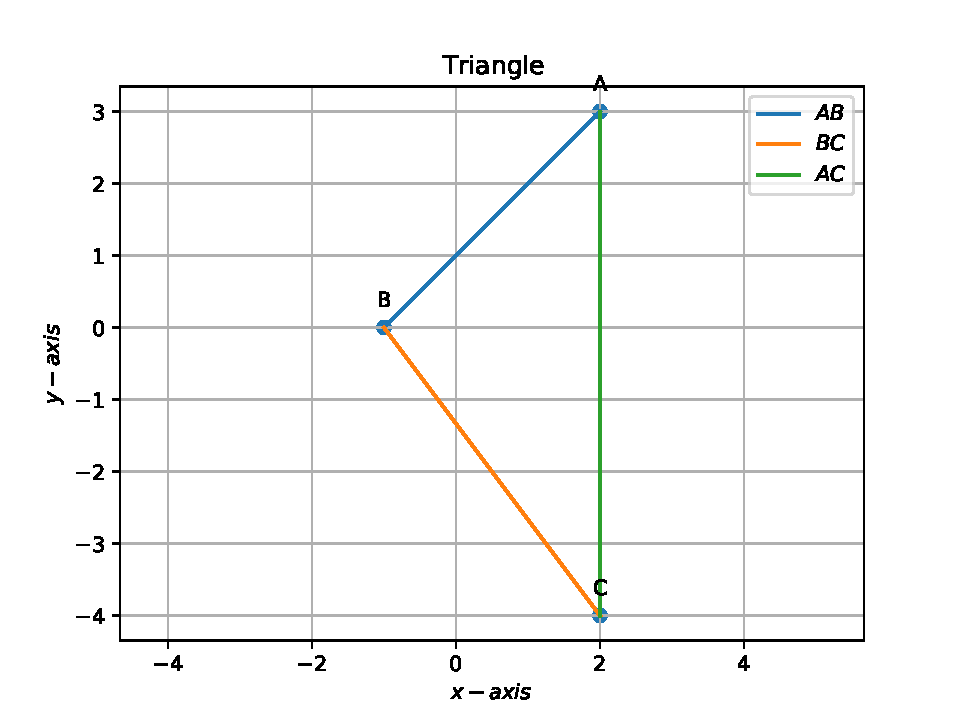
\includegraphics[width=\columnwidth]{./figs/problem1a.pdf}
	\end{center}
\caption{}
\label{fig:Fig1}
\end{figure}

\item $(–5, –1), (3, –5), (5, 2)$ \\ 
\solution The area of the triangle with vertices $\vec{A}, \vec{B}, \vec{C}$ is given by  
  \label{prop:area2e}
  \begin{align}
    \label{eq:area2e}
	\frac{1}{2}\norm{\brak{\vec{A}-\vec{B}} \times \brak{\vec{A}-\vec{C}}}
 = 
 \frac{1}{2}\norm{\vec{A} \times \vec{B}+\vec{B} \times \vec{C}+\vec{C} \times \vec{A}}
\end{align}

The value of the cross product of two vectors is given by \\

\begin{align}
  \label{eq:det2e}
  \mydet{\vec{M}} &= \mydet{\vec{A} & \vec{B}} 
  \\
  &= \mydet{a_1 & b_1\\a_2 & b_2} = a_1b_2 - a_2 b_1
\end{align}

		Therefore, \eqref{eq:area2e} equals \\
\begin{align}
	\text{Area} &=	\frac{1}{2}\brak{a_1b_2 - a_2 b_1 + b_1c_2 - b_2 c_1 + c_1a_2 - c_2 a_1}  \\
	&=	\frac{1}{2}\brak{\brak{-5} \times \brak{-5} - \brak{-1} \times 3 + 3 \times 2 - \brak{-5} \times 5 + \brak{-1} \times 5 - \brak{-5} \times 2}  \\
	&=\frac{1}{2}\brak{25 + 3  + 6 + 25 - 5 + 10} \\
	&=\frac{1}{2}\brak{64}  \\
	&=32 \text{ Sq units}	       
\end{align}

\begin{figure}[!h]
	\begin{center}
		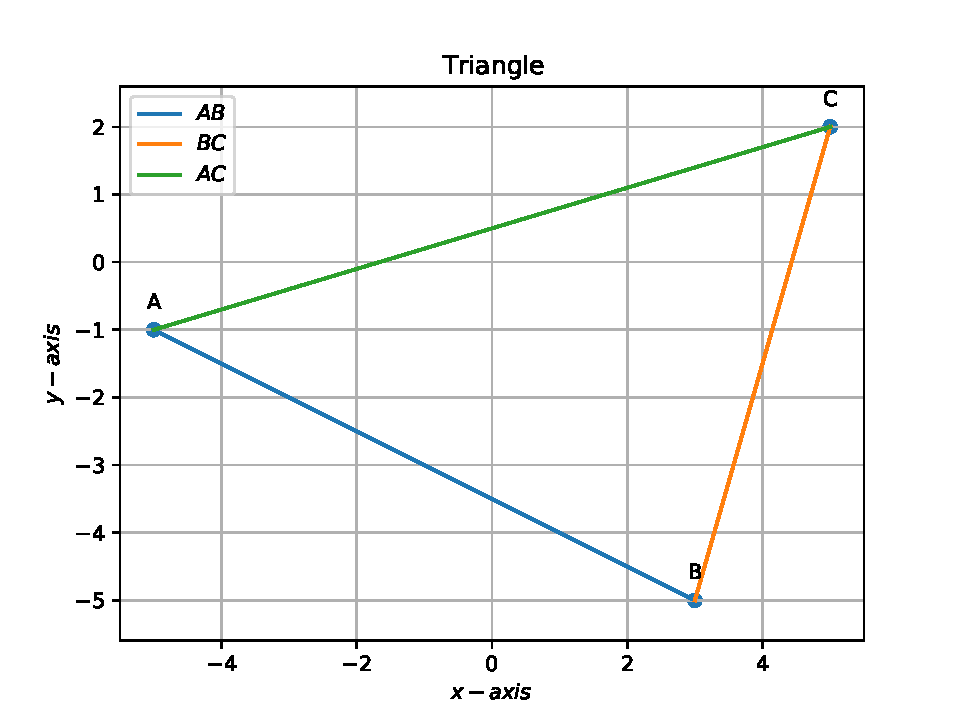
\includegraphics[width=\columnwidth]{./figs/problem1b.pdf}
	\end{center}
\caption{}
\label{fig:Fig2}
\end{figure}
\end{enumerate}

\end{enumerate}


\end{document}
